\chapter{Multi-period optimal power flow (TCOPFLOW)}\label{chap:tcopflow}
\todo

\section{Formulation}
The multi-period optimal power flow problem is a series of optimal power flow problems coupled via temporal constraints. The generator real power deviation ($p_{jt}^{\text{g}} - p_{jt-\Delta{t}}^{\text{g}}$) constrained within the ramp limits form the temporal constraints. An illustration of the temporal constraints is shown in Fig. \ref{fig:tcopflow} with four time steps. Each time-step $t$ is coupled with its preceding time $t-\Delta{t}$, where $\Delta{t}$ is the time-step where the objective is to find a least cost dispatch for the given time horizon.

\definecolor{lavander}{cmyk}{0,0.48,0,0}
\definecolor{violet}{cmyk}{0.79,0.88,0,0}
\definecolor{burntorange}{cmyk}{0,0.52,1,0}

\def\lav{lavander!90}
\def\oran{orange!30}

\tikzstyle{time}=[draw,circle,violet,bottom color=\lav,
                  top color= white, text=violet,minimum width=20pt]
\tikzstyle{base}=[draw,circle,burntorange, left color=\oran,
                       text=violet,minimum width=20pt]

\begin{figure}[h!]
\centering
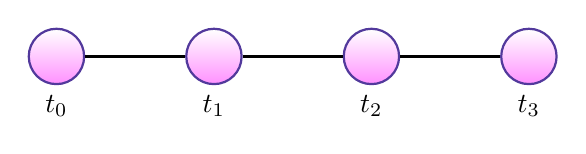
\begin{tikzpicture}[auto, thick]
  \node[time,label=below:$t_0$] (t0) at (0,0) {};
  \node[time,label=below:$t_1$] (t1) at (2,0) {};
  \node[time,label=below:$t_2$] (t2) at (4,0) {};
  \node[time,label=below:$t_3$] (t3) at (6,0) {};
  
  \path (t0) edge (t1);
  \path (t1) edge (t2);
  \path (t2) edge (t3);


\end{tikzpicture}
\caption{Multi-period optimal power flow example with four time-steps. The lines connecting the different time-periods denote the coupling between them.}
\label{fig:tcopflow}
\end{figure}


In general form, the equations for multi-period optimal power flow are given by
(\ref{eq:tcopflow_start}) -- (\ref{eq:tcopflow_end}). TCOPFLOW solves to minimize the total generation cost $\sum_{t=0}^{N_t-1}f(x_t)$ over the time horizon, where $N_t$ is the number of time-steps. At each time-step, the equality constraints ($g(x_t)$), inequality $h(x_t)$, and the lower/upper limit ($x^-$,$x^+$) constraints need to be satisfied. Equation (\ref{eq:tcopflow_end}) represents the coupling between the consecutive time-steps. It is a most common form of coupling that limits the deviation of the real power generation at time $t$ from its preceding time-step $t-\Delta{t}$ to within its ramping capability $\delta_t{x}$.


\begin{align}
\centering
\text{min}&~\sum_{t=0}^{N_t-1} f(x_t) &  \label{eq:tcopflow_start}\\
&\text{s.t.}& \nonumber \\
&~g(x_t) = 0,                                        &t \in \left[0,N_t-1\right]& \\
&~h(x_t) \le 0,                                      &t \in \left[0,N_t-1\right]& \\
x^- & \le x_t \le x^+,                               &t\in \left[0,N_t-1\right]& \\
-\delta_t{x} & \le x_t - x_{t-\Delta{t}} \le \delta_t{x},&t \in \left[1,N_t-1\right]&
\label{eq:tcopflow_end}
\end{align}

\section{Input and Output}
\begin{itemize}
    \item \textbf{Network file:} The network file describing the network details. Only \matpower format files are currently supported.
    \item \textbf{Load data:} One file for load real power and one fo reactive power. The files need to be in CSV format. An example of the format for the 9-bus case is \href{https://gitlab.pnnl.gov/exasgd/frameworks/exago/-/tree/master/datafiles/case9}{here}.
    \item \textbf{Wind generation:} The wind generation time-series described in CSV format. See an example of the format \href{https://gitlab.pnnl.gov/exasgd/frameworks/exago/-/tree/master/datafiles/case9}{here}.
\end{itemize}


The \tcopflow output is saved to a directory named \emph{tcopflowout}. This directory contains $N_t$ files, one for each time-step, in \matpower data file format.

\section{Solvers}
\section{Usage}
\todo
\section{Options}
\todo
\section{Examples}
\todo